\chapter{Etude préalable}

\minitocsection

\section*{Introduction}
\addcontentsline{toc}{section}{Introduction}
Ce chapitre présente l'état actuel de la gestion logistique chez Poulina Group Holding, dresse un état de l'art des principales applications commerciales de gestion de flotte et en identifie les limites vis-à-vis des contraintes spécifiques de PGH. Il expose enfin les raisons pour lesquelles le développement sur mesure de Fleet~AI s'impose comme la seule solution viable.

% =============================================================
\section{Etude de l'existant}
% =============================================================

\subsection{Description des procédures actuelles}

Chez Poulina Group Holding, la gestion logistique repose intégralement sur des procédés manuels : un seul planificateur répartit les missions par téléphone, sans système centralisé. Les principales limites observées sont :

\begin{itemize}
  \item Aucune visibilité sur les commandes en attente ni priorisation objective.
  \item Itinéraires construits empiriquement, sans optimisation ni suivi GPS.
  \item Preuves de livraison informelles : pas de signature numérique, pas de photo horodatée.
  \item Encaissements non rapprochés automatiquement avec les commandes correspondantes.
  \item Absence de données opérationnelles exploitables : tout incident disparaît sans être tracé.
\end{itemize}

\subsection{Etude comparative des solutions existantes}

La gestion de flotte est un domaine couvert par plusieurs plateformes commerciales. Pour identifier les meilleures pratiques et évaluer leur adéquation aux besoins de PGH, nous avons étudié trois applications majeures : \textbf{Geotab}, \textbf{Samsara} et \textbf{Verizon Connect}.

\subsubsection*{Geotab}
Geotab est une plateforme très orientée télématique véhiculaire. Elle propose un suivi GPS avancé, des rapports de conduite détaillés et une intégration avec de nombreux partenaires via une marketplace ouverte. Sa forte dépendance aux boîtiers OBD physiques complique cependant le déploiement rapide sur une flotte hétérogène, et son interface nécessite une formation approfondie.

\begin{figure}[H]
\centering
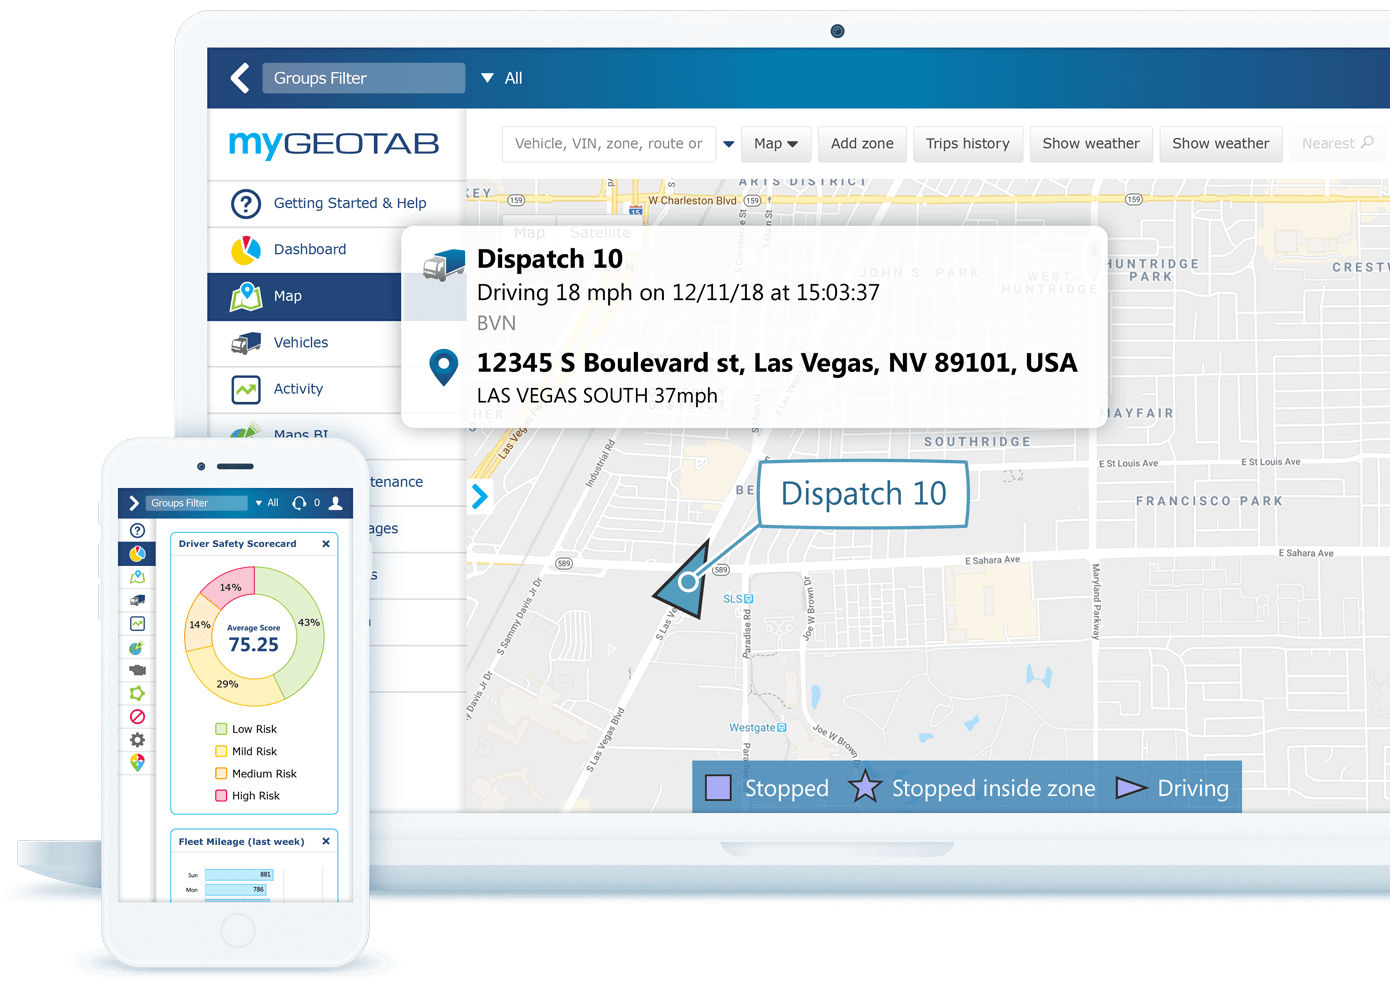
\includegraphics[width=0.85\linewidth]{img/geotab_screenshot}
\caption{Interface de la plateforme Geotab --- tableau de bord de suivi de flotte}
\label{fig:geotab-screenshot}
\end{figure}

\subsubsection*{Samsara}
Samsara est considérée comme l'une des plateformes les plus complètes du marché. Elle se distingue par l'intégration de caméras IA embarquées, un suivi GPS performant et des outils analytiques avancés. Néanmoins, la dépendance matérielle (caméras IA embarquées) constitue un frein logistique majeur pour un déploiement en Tunisie.

\begin{figure}[H]
\centering
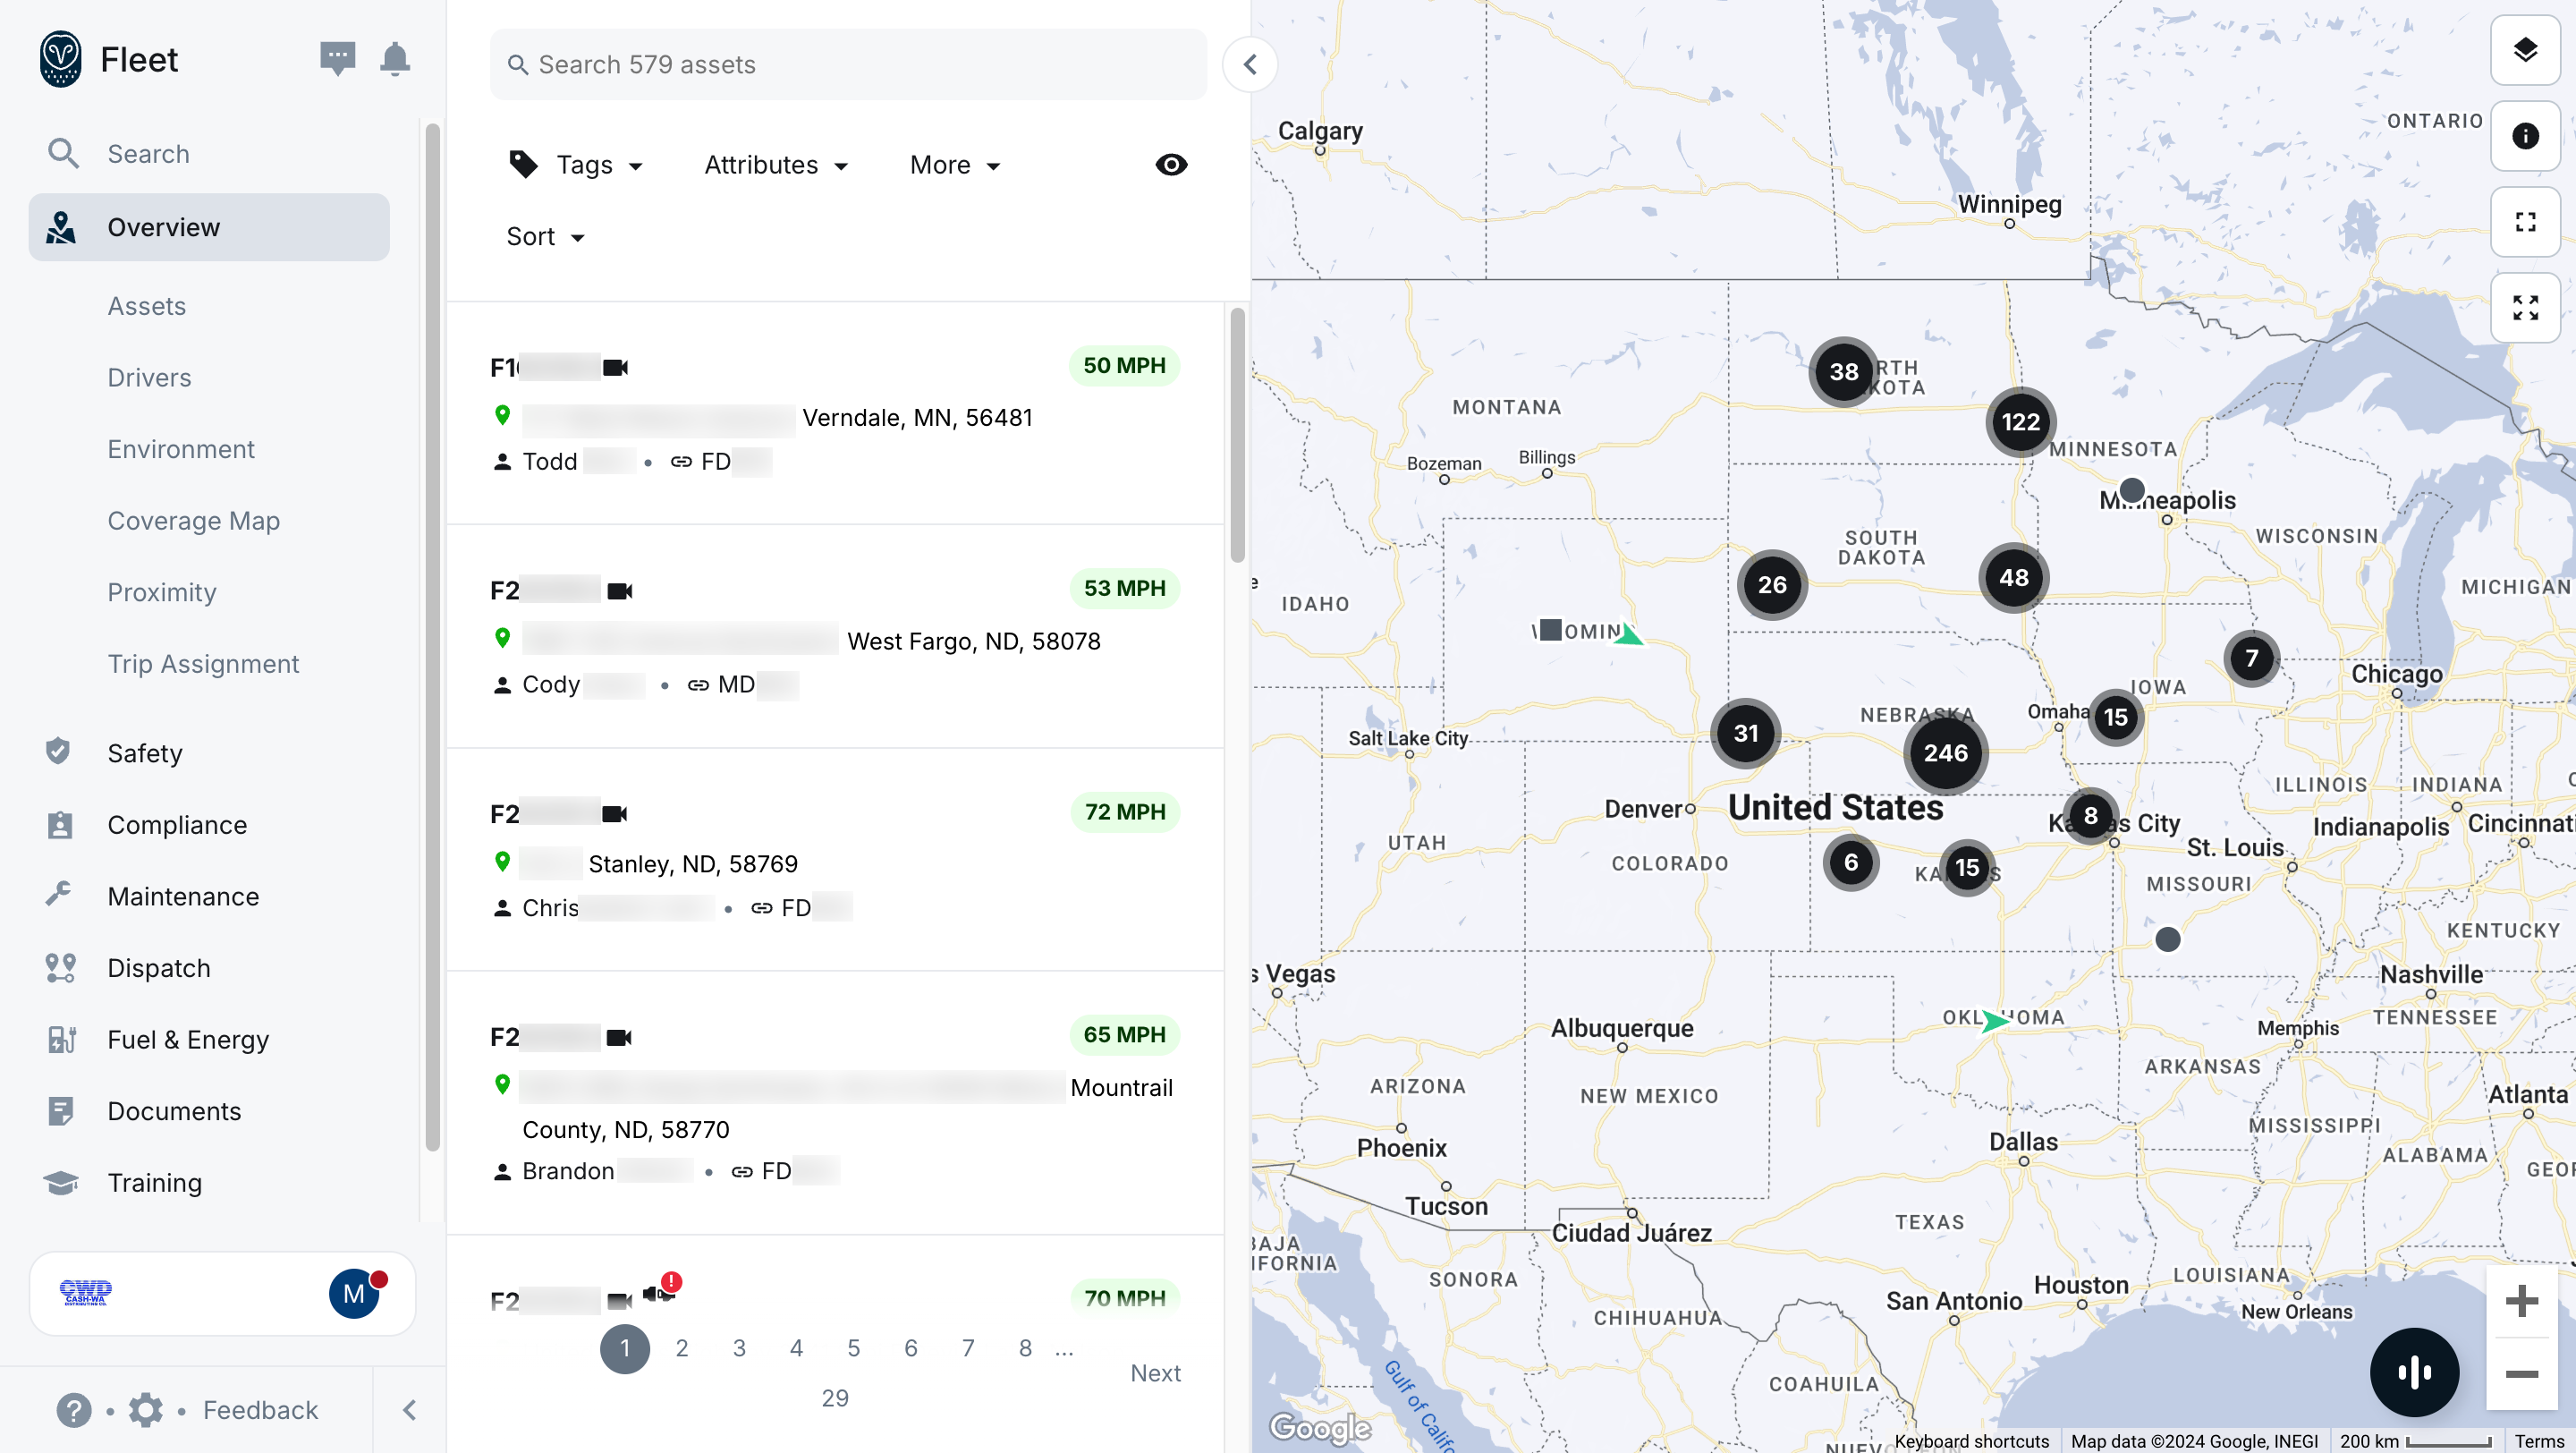
\includegraphics[width=0.85\linewidth]{img/samsara_screenshot}
\caption{Interface de la plateforme Samsara --- tableau de bord analytique}
\label{fig:samsara-screenshot}
\end{figure}

\subsubsection*{Verizon Connect}
Verizon Connect intègre un suivi GPS standard, la gestion des conducteurs et des alertes automatiques. Ses fonctionnalités analytiques manquent cependant de profondeur, et son API s'avère trop limitée pour une intégration poussée avec des systèmes d'information tiers.

\begin{figure}[H]
\centering
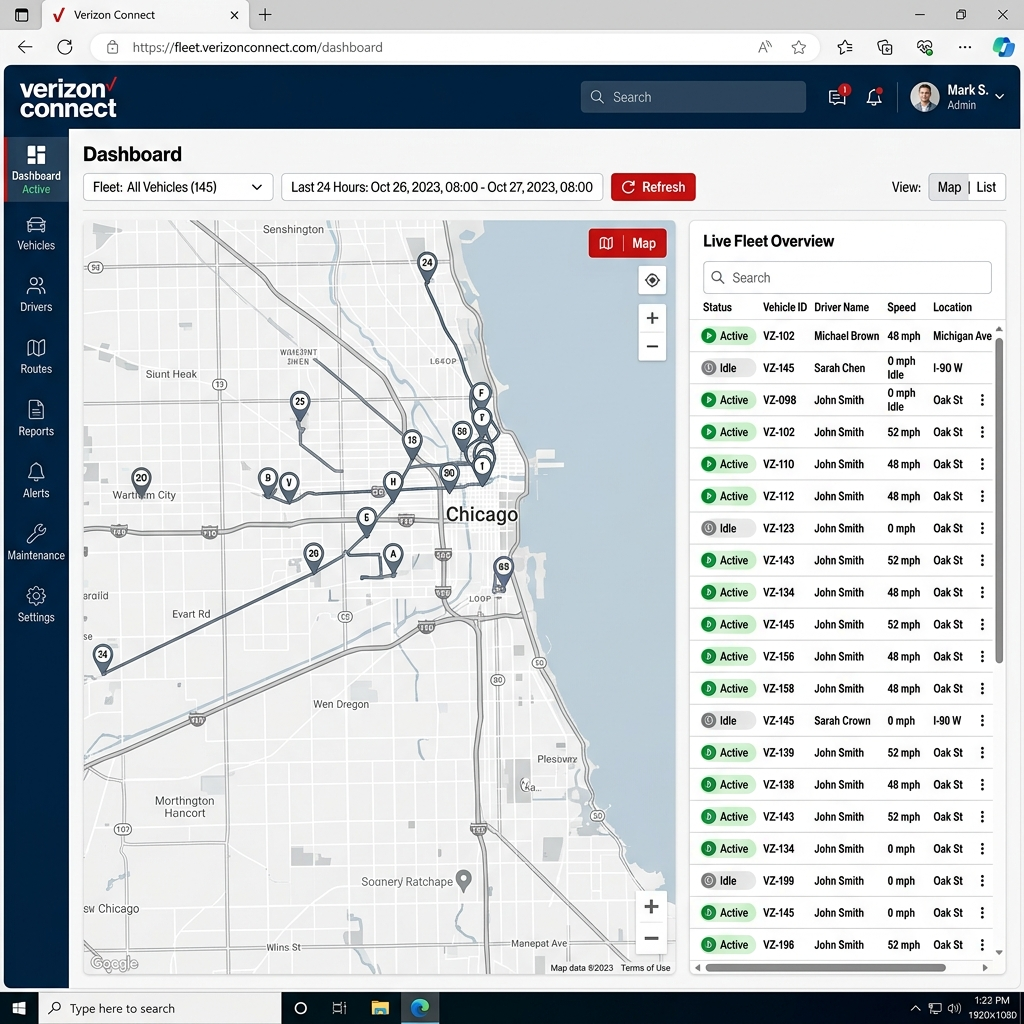
\includegraphics[width=0.85\linewidth]{img/verizon_screenshot}
\caption{Interface de la plateforme Verizon Connect --- vue de suivi des véhicules}
\label{fig:verizon-screenshot}
\end{figure}

\subsubsection*{Comparaison des fonctionnalités}
Le tableau ci-dessous synthétise les fonctionnalités offertes par ces trois applications.

\setlength{\arrayrulewidth}{1pt}
\begin{longtable}{|>{\raggedright\arraybackslash}p{3.5cm}|>{\raggedright\arraybackslash}p{3.5cm}|>{\raggedright\arraybackslash}p{3.5cm}|>{\raggedright\arraybackslash}p{3.5cm}|}
  \hline
  \rowcolor{headerbg}
  \textbf{Fonctionnalité} & \textbf{Geotab} & \textbf{Samsara} & \textbf{Verizon Connect} \\
  \hline
  \endfirsthead

  \hline
  \rowcolor{headerbg}
  \textbf{Fonctionnalité} & \textbf{Geotab} & \textbf{Samsara} & \textbf{Verizon Connect} \\
  \hline
  \endhead

  Suivi GPS temps réel & Oui, très avancé & Oui, intégré & Oui \\
  \hline
  Gestion des chauffeurs & Basique & Avancée (caméra IA) & Basique \\
  \hline
  Gestion des véhicules & Complète & Complète & Complète \\
  \hline
  Zones géographiques & Oui (géofencing) & Oui (géofencing) & Oui (géofencing) \\
  \hline
  Tableau de bord & Personnalisable & Moderne et intuitif & Standard \\
  \hline
  Gestion des coûts & Via marketplace & Intégrée & Basique \\
  \hline
  Contrôle d'accès (RBAC) & Limité & Basique & Limité \\
  \hline
  Intégration ERP/SI & API ouverte & API ouverte & API limitée \\
  \hline
  Audit/Traçabilité & Limité & Partiel & Limité \\
  \hline
  Hébergement & Cloud uniquement & Cloud uniquement & Cloud uniquement \\
  \hline
\caption{Comparaison des applications de gestion de flotte existantes}
\end{longtable}
\setlength{\arrayrulewidth}{0.4pt}

% =============================================================
\section{Critique de l'existant}
% =============================================================

L'analyse du fonctionnement actuel chez PGH et l'étude des solutions commerciales disponibles font apparaître des lacunes structurelles qui justifient pleinement le développement d'une solution sur mesure.

\subsubsection*{Limites organisationnelles du système actuel :}
\begin{itemize}
  \item La concentration de la planification sur un seul acteur crée un point de défaillance unique et limite la capacité de traitement lors des pics d'activité.
  \item La communication orale entre planificateur et chauffeurs génère des pertes d'information et une absence totale de traçabilité des échanges.
  \item L'absence d'optimisation des itinéraires entraîne une consommation excessive de carburant et un non-respect fréquent des créneaux horaires contractuels.
  \item Sans suivi GPS ni preuve de livraison numérique, il est impossible de détecter les retards, de résoudre les litiges ou de garantir la conformité des remises de marchandises.
  \item L'informalité des encaissements expose l'entreprise à des risques financiers et à des écarts comptables non détectés.
\end{itemize}

\subsubsection*{Incompatibilités des solutions commerciales étudiées :}
\begin{itemize}
  \item[$\bullet$] \textbf{Hébergement cloud exclusif :} Ces applications fonctionnent uniquement en mode SaaS, ce qui pose des problèmes critiques de souveraineté des données pour PGH, qui exige un déploiement on-premise.
  \item[$\bullet$] \textbf{Coût prohibitif :} Les tarifications par abonnement mensuel et par véhicule sont inadaptées à l'échelle de la flotte de PGH.
  \item[$\bullet$] \textbf{Absence d'intégration WFMS :} Aucune solution ne propose d'intégration native avec la plateforme WFMS du groupe ; des développements middleware coûteux seraient nécessaires.
  \item[$\bullet$] \textbf{Contrôle d'accès inadapté :} Les systèmes de permissions ne correspondent pas à la hiérarchie spécifique requise par PGH (Administrateur, Planificateur, Manager, Chauffeur, Responsable Engagement Client -- REC, Client).
  \item[$\bullet$] \textbf{Disponibilité locale limitée :} Le support technique en Tunisie de ces éditeurs internationaux est insuffisant pour garantir une continuité de service critique.
\end{itemize}

Ces constats démontrent qu'aucune solution du marché ne peut répondre simultanément aux exigences de déploiement on-premise, d'intégration WFMS, de contrôle d'accès hiérarchique et de couverture fonctionnelle métier propres à PGH. Le développement sur mesure de Fleet~AI s'impose donc comme la seule approche viable.

% =============================================================
\section{Solution proposée}
% =============================================================

Face à ces limites, PGH a fait le choix stratégique du développement sur mesure avec la création de \textbf{Fleet~AI} par GREPSYS. Cette solution est déployée directement sur les serveurs de PGH (on-premise) et s'intègre nativement à la plateforme WFMS existante, sans en modifier le code source.

Fleet~AI couvre l'ensemble du cycle logistique à travers cinq modules principaux :

\begin{itemize}
  \item La planification assistée avec optimisation algorithmique des itinéraires et affectation guidée.
  \item Une application mobile pour les chauffeurs garantissant la collecte de preuves de livraison numériques et supportant un mode hors-ligne.
  \item L'intégration de modèles d'intelligence artificielle pour prédire la demande par zone et anticiper les retards de livraison.
  \item La mise en place de tableaux de bord décisionnels et de KPIs centralisés à l'échelle du holding.
  \item La gestion numérisée des paiements et des réclamations avec traçabilité complète de chaque opération terrain.
\end{itemize}

\section*{Conclusion}
\addcontentsline{toc}{section}{Conclusion}
L'étude de l'existant a mis en évidence qu'aucune plateforme du marché, telles que Geotab, Samsara ou Verizon Connect, ne pouvait répondre aux exigences de PGH. Leurs limites en matière de coût, de déploiement cloud (SaaS), d'intégration au WFMS et de gestion des rôles les rendent inadaptées. C'est pourquoi le développement sur mesure de Fleet~AI s'est imposé comme la seule approche viable. Le chapitre suivant détaille la méthodologie et l'architecture adoptées pour concrétiser cette solution.
